\documentclass{article}

% Recommended, but optional, packages for figures and better typesetting:
\usepackage{microtype}
\usepackage{graphicx}
\usepackage{subfigure}
\usepackage{booktabs} % for professional tables

% hyperref makes hyperlinks in the resulting PDF.
% If your build breaks (sometimes temporarily if a hyperlink spans a page)
% please comment out the following usepackage line and replace
% \usepackage{icml2020} with \usepackage[nohyperref]{icml2020} above.
\usepackage{hyperref}
\graphicspath{{figures/}}
\usepackage{amsmath,amsthm,amssymb}
\newtheorem{theorem}{Theorem}
\newtheorem{lemma}{Lemma}
\usepackage{bm}
\newcommand{\vect}[1]{\boldsymbol{\mathbf{#1}}}

% Attempt to make hyperref and algorithmic work together better:
\newcommand{\theHalgorithm}{\arabic{algorithm}}

% Use the following line for the initial blind version submitted for review:
\usepackage{icml2020}

% If accepted, instead use the following line for the camera-ready submission:
% \usepackage[accepted]{icml2020}


% The \icmltitle you define below is probably too long as a header.
% Therefore, a short form for the running title is supplied here:
\icmltitlerunning{Submission and Formatting Instructions for ICML 2020}

\begin{document}

\twocolumn[
\icmltitle{On the connection between stochastic optimization and splitting scheme for ODE.}

% It is OKAY to include author information, even for blind
% submissions: the style file will automatically remove it for you
% unless you've provided the [accepted] option to the icml2020
% package.

% List of affiliations: The first argument should be a (short)
% identifier you will use later to specify author affiliations
% Academic affiliations should list Department, University, City, Region, Country
% Industry affiliations should list Company, City, Region, Country

% You can specify symbols, otherwise they are numbered in order.
% Ideally, you should not use this facility. Affiliations will be numbered
% in order of appearance and this is the preferred way.
\icmlsetsymbol{equal}{*}

\begin{icmlauthorlist}
\icmlauthor{Daniil Merkulov}{sk}
\icmlauthor{Ivan Oseledets}{sk}
\end{icmlauthorlist}

\icmlaffiliation{sk}{Center for Computational and Data-Intensive Science and Engineering, Skolkovo Institute of Science and Technology, Moscow, Russia}

\icmlcorrespondingauthor{Daniil Merkulov}{daniil.merkulov@skoltech.ru}
\icmlcorrespondingauthor{Ivan Oseledets}{i.oseledets@skoltech.ru}

% You may provide any keywords that you
% find helpful for describing your paper; these are used to populate
% the "keywords" metadata in the PDF but will not be shown in the document
\icmlkeywords{Stochastic gradient descent, ordinary differential equations, splitting scheme, Kaczmarz method, Optimization}

\vskip 0.3in
]

% this must go after the closing bracket ] following \twocolumn[ ...

% This command actually creates the footnote in the first column
% listing the affiliations and the copyright notice.
% The command takes one argument, which is text to display at the start of the footnote.
% The \icmlEqualContribution command is standard text for equal contribution.
% Remove it (just {}) if you do not need this facility.

\printAffiliationsAndNotice{}  % leave blank if no need to mention equal contribution
% \printAffiliationsAndNotice{\icmlEqualContribution} % otherwise use the standard text.

\begin{abstract}
We present different view on stochastic optimization, which goes back to the splitting schemes for approximate solutions of ODE. In this work we provide a connection between stochastic gradient descent approach and first order splitting scheme for ODE. We present, that the Kaczmarz method is the limit case of the splitting scheme for unitary batch SGD linear least squares approach. We support our findings with empirical tests.
\end{abstract}

\section{Introduction}
A lot of practical problems arising in machine learning require minimization of a finite sample average which can be written in the form
\begin{equation}\label{strang:finitesum}
    f(\vect{\vect{\theta}}) = \frac{1}{n} \sum_{i=1}^n f_i(\vect{\vect{\theta}}) \rightarrow \min_{\vect{\vect{\theta}} \in \mathbb{R}^p},
\end{equation}
where the sum goes over the \emph{minibatches} of the original dataset. Vanilla stochastic gradient descent (SGD) method \cite{robbins1951stochastic} consists sequential steps in the direction of the gradient of $f_i(\vect{\theta})$, where $i$ is to be chosen randomly from $1$ to $n$ without replacement.
\begin{equation}
\vect{\theta}_{k+1} = \vect{\theta}_{k} - h_{k} \nabla f_i.
\end{equation}
Gradient descent method can be considered as an Euler discretization of the ordinary differential equation (ODE) of the form of the gradient flow
\begin{equation}\label{strang:euler}
    \frac{d \vect{\theta}}{d t} = -\nabla f(\vect{\theta}).
\end{equation}
In continuous time, SGD if often analyzed by introducing a noise into the right-hand side of \eqref{strang:euler}. However, for real dataset the distribution of the noise obtained by replacing the full gradient by its minibatch variant is not known and can be different for different problems. Instead, we propose a new view on the SGD as a \emph{first-order splitting scheme} for \eqref{strang:euler}, thus shedding a new light on SGD-type algorithms. This representation allows to use more efficient splitting schemes for the approximation of the full gradient flow. We show, that second-order Marchuk/Strang splitting scheme (\cite{marchuk1968some}, \cite{strang1968construction}) provides faster convergence 

% We'll leave SAG for a moment.. Moreover, we interpret stochastic average gradient (SAG)\cite{schmidt2017minimizing} approach as the \emph{splitting scheme with rebalancing} of the SAG method, which we call \emph{SAG2} method. In implementation, the second-order scheme consists in a sequential processing of minibatches first from $1$ to $m$, and then from $m$ to $1$, i.e. a single iteration of SAG2 has the same cost as two iterations of SAG.

\textbf{Contributions}
\begin{itemize}
    \item We show, that vanilla SGD could be considered as a splitting scheme for a full gradient flow.
    \item We demonstrate the connection between rebalancing splitting and stochastic average gradient method.
    \item We propose new optimization method, SAG2 based on second order splitting scheme and show that it gives better convergence, than the standard SAG method.
    % Перспективные вещи - аналитическая связь размера батча и величины шага, устойчивость к шагу
\end{itemize}

%================================================
% SGD as a splitting scheme
%================================================

\section{SGD as a splitting scheme}

We want to establish the connection between splitting scheme for ODE and stochastic optimization. In this section we firstly consider simple ODE, where we can apply splitting idea and corresponding minimization problem.

\subsection{Splitting schemes for ODEs}
The best example to start from is simple ODE with right-hand-side, consisting of two summands:
\begin{equation}
    \frac{d \vect{\theta}}{d t} = - \frac{1}{2} \left( g_1(\vect{\theta}) + g_2(\vect{\theta})\right)
    \label{strang:gradientflow}
\end{equation}
Suppose, we want to find the solution $\vect{\theta}(h)$ of \eqref{strang:gradientflow} via integrating it on the small timestep $h$. The first order splitting scheme defined by solving first:
$$
\frac{d \vect{\theta}}{d t} = - \frac{1}{2} g_1(\vect{\theta}), \quad \vect{\theta}(0) = \vect{\theta}_0
$$
with exact solution $\vect{\theta}_1(h)$ at the moment $h$ , followed by
$$
\frac{d \vect{\theta}}{d t} = - \frac{1}{2} g_2(\vect{\theta}), \quad \vect{\theta}(0) = \vect{\theta}_1(h)
$$
with exact solution $\vect{\theta}_2(h)$ at the moment $h$. Thus, the first order approximation could be written as a combinations of both solutions:
$$
\vect{\theta}^I(h) = \vect{\theta}_2(h) \circ \vect{\theta}_1(h) \circ \vect{\theta}_0,
$$
while the second order scheme takes 3 substeps:
$$
\vect{\theta}^{II}(h) = \vect{\theta}_1\left(\frac{h}{2}\right) \circ \vect{\theta}_2(h) \circ \vect{\theta}_1\left(\frac{h}{2}\right) \circ \vect{\theta}_0
$$
Order of scheme defines the degree of polynomial of $h$, up to which the true solution and approximation are coincide. The local error of both schemes is given by Baker - Campbell - Hausdorff formula (\cite{baker1901further}, \cite{campbell1896law}, \cite{hausdorff1906symbolische}) (see \cite{macnamara2016operator} for the details)
\begin{equation}
    \label{strang:lie_error}
    \vect{\theta}^I(h) - \vect{\theta}(h) = \frac{h^2}{2} \left[g_{1}, g_{2}\right]  + \mathcal{O}(h^3),
\end{equation}
\begin{equation}
    \label{strang:marchuk_error}
    \begin{split}
    &\vect{\theta}^{II}(h) - \vect{\theta}(h) =\\&= \frac{h^{3}}{24} \left([[g_1, g_2], g_1]+2[[g_1, g_2], g_2]\right)+\mathcal{O}\left(h^{4}\right)
    \end{split}
\end{equation}

where $\left[ g_1, g_2\right] = \frac{d g_1}{d \vect{\theta}} g_2 - \frac{d g_2}{d \vect{\theta}} g_1 $ stands for commutator of the vector fields $g_1$ and $g_2$. The $\vect{\theta}_0 = \vect{\theta}(0)$ for initial condition of original ODE.

Note, that the basic idea of splitting could be also applied, when the number of terms in the right-hand side of ODE is greater, than two. In this case splitting scheme will take the following form:
\begin{equation}\label{strang:marchuk}
	\vect{\theta}^I(h) = \vect{\theta}_m(h) \circ \vect{\theta}_{m-1} \circ \ldots \circ \vect{\theta}_2(h) \circ \vect{\theta}_1(h) \circ \vect{\theta}_0
\end{equation}
\begin{equation}\label{strang:strang}
\begin{split}
	\vect{\theta}^{II}(h) = \vect{\theta}_1\left(\frac{h}{2}\right) \circ \vect{\theta}_2\left(\frac{h}{2}\right) \circ\ldots \vect{\theta}_m(h) \circ \ldots \\ \ldots \circ \vect{\theta}_2\left(\frac{h}{2}\right)  \circ \vect{\theta}_1\left(\frac{h}{2}\right) \circ \vect{\theta}_0
\end{split}
\end{equation}

\subsection{SGD as approximation for the Gradient Flow equation}
Now we consider classical SGD method as a splitting scheme for the full gradient descent (\cite{cauchy1847methode}). Suppose, we have the simplest ($m=2$) finite sum minimization problem:
$$
\min_{\vect{\theta} \in \mathbb{R}^n} \frac{1}{m}\sum\limits_{i=1}^m f_i(\vect{\theta}) = \min_{\vect{\theta} \in \mathbb{R}^n} \frac{1}{2} \left( f_1(\vect{\theta}) + f_2(\vect{\theta})\right)
$$
Let us denote by $g_i^k = \nabla f_i(\vect{\theta}_k)$, than, the vanilla gradient descent will be written as
$$
\vect{\theta}_{k+1} = \vect{\theta}_k - h\cdot\frac{1}{2} \left( g^k_1 + g^k_2\right),
$$
while SGD version will take steps iteratively over minibatch gradient directions:
\begin{align*}\label{strang:sgd2}
\vect{\theta}_{k+1} &= \vect{\theta}_k - h\cdot g^k_1 \\
\vect{\theta}_{k+2} &= \vect{\theta}_{k+1} - h\cdot  g^{k+1}_2
\end{align*}
These two iterations forms an epoch in SGD approach. Each of the substeps can be considered as a forward Euler method for the discretization of the ODE for a timestep $h$
\begin{align*}
    \frac{d \vect{\theta}^I}{d t} = -g_1, \quad \vect{\theta}^I(0) = \vect{\theta}_{k},\\
    \frac{d \vect{\theta}^{II}}{d t} = -g_2, \quad \vect{\theta}^{II}(0) = \vect{\theta}^{I}(h),
\end{align*}
therefore the final result for a sufficiently small $h$ approximates the gradient flow for at time $t + h$. The vanilla gradient descent, however, is only approximating the gradient flow at time $t + h/2$. For larger number of minibatches, rather then the GD flow. One can notice, that in SGD we use a very simple time integration inside the substep. In some cases, we can integrate the subproblem exactly, without using forward Euler scheme. Generalized linear models are among such problems, but we will first study the linear least squares case in more details, since in this case we can obtain non-trivial error bounds.

\subsection{Splitting approximation for the Gradient Flow equation}

It is interesting to look how the pure splitting scheme corresponds to the SGD approach. For this purpose we consider illustrative example of Gradient Flow equation \ref{strang:simple_GF}, where the right-hand side of ODE is just the sum of operators acting on $\vect{\theta}$, which allows us to apply splitting scheme approximation directly.
\begin{equation}
\label{strang:simple_GF}
\frac{d \vect{\theta}}{d t} = -\frac{1}{2} \sum\limits_{i=1}^2 \nabla f_i (\vect{\theta}) = - \frac{1}{2} \nabla f_1 (\vect{\theta}) -\frac{1}{2}  \nabla f_2 (\vect{\theta})
\end{equation}

In order to establish the connection between splitting scheme and SGD we use the Euler discretization below:

\begin{align*}
% \label{strang:simple_GF_splitting}
&\qquad\text{Splitting step} &\text{Euler discretization} \\
&\frac{d \vect{\theta}}{d t} = -\frac{1}{2}\nabla f_1(\vect{\theta}) &\tilde{\vect{\theta}}_{I} = \vect{\theta}_0 - \frac{h}{2}\nabla f_1 (\vect{\theta}_0) \\
&\frac{d \vect{\theta}}{d t} = -\frac{1}{2}\nabla f_2(\vect{\theta}) &\vect{\theta}_{I} = \tilde{\vect{\theta}}_{I} - \frac{h}{2}\nabla f_2 (\tilde{\vect{\theta}}_{I})
\end{align*}


\begin{align*}
% \label{strang:simple_GF_splitting}
&\qquad\text{SGD epoch} &\text{First order splitting} \\
&\tilde{\vect{\theta}}_{SGD} = \vect{\theta}_0 - h \nabla f_1 (\vect{\theta}_0) &\tilde{\vect{\theta}}_{I} = \vect{\theta}_0 - \frac{h}{2}\nabla f_1 (\vect{\theta}_0) \\
&\vect{\theta}_{SGD} = \tilde{\vect{\theta}}_{SGD} - h \nabla f_2 (\tilde{\vect{\theta}}_{SGD}) &\vect{\theta}_{I} = \tilde{\vect{\theta}}_{I} - \frac{h}{2}\nabla f_2 (\tilde{\vect{\theta}}_{I})
\end{align*}

Thus, we can conclude, that \textit{one epoch of SGD is just the splitting scheme for the discretized Gradient Flow ODE with $2 \cdot h$ step size ($m \cdot h$ in case of $m$ batches)}

This idea gives additional intuition on the method. Both approaches are solving local problems through the Euler discretization. Given an information about the Euler scheme limitation, why not solve these local problems more accurate? While Euler's scheme is first order accurate, there is no point in using higher order splitting scheme's in such setting. Therefore, total error is defined by the accuracy of splitting and local problem integration. We should improve them both to achieve gain.

%================================================
% Applications
%================================================

\section{Applications}
\subsection{Linear least squares}
\subsubsection{Problem}
Let $f_i(\vect{\theta}) = \Vert \vect{x_i}^{\top} \vect{\theta} - y_i \Vert^2$, then problem \eqref{strang:finitesum} is the linear least squares problem, which can be written as
\begin{equation}\label{strang:LLS}
   f(\vect{\theta}) = \frac{1}{n}\Vert X \vect{\theta} - \vect{y} \Vert_2^2  = \frac{1}{n}\sum\limits_{i=1}^s\Vert X_i \vect{\theta} - \vect{y_i} \Vert_2^2\to \min_{\vect{\theta} \in \mathbb{R}^p},
\end{equation}
where $X \in \mathbb{R}^{n \times p}$ and $\vect{y} \in \mathbb{R}^p$ and the second part of the equation stands for $s$ mini-batches with size $b$ regrouping ($b \cdot s = n$): $X_i \in \mathbb{R}^{b \times p}, \vect{y_i} \in \mathbb{R}^{b}$

\begin{equation}\label{strang:LLS_grad}
\nabla_\theta f(\vect{\theta}) = \nabla f(\vect{\theta}) = \frac{1}{n}\sum\limits_{i=1}^s X_i^\top(X_i \vect{\theta} - \vect{y_i})
\end{equation}

The gradient flow equation will be written as follows:
\begin{equation}\label{strang:LLS_GF}
\frac{d \vect{\theta}}{d t} = - \frac{1}{n}\sum\limits_{i=1}^s X_i^\top( X_i \vect{\theta} - \vect{y_i})
\end{equation}

\subsubsection{Exact solution of the local problem}
On each splitting approximation step we need to solve the local problem:
\begin{equation}\label{strang:LLS_local_problem}
\frac{d \vect{\theta}}{d t} = - \frac{1}{n}X_i^\top(X_i \vect{\theta} - \vect{y_i})
\end{equation}
\begin{theorem}\label{strang:LLS_local_solution} For any matrix $\vect{x_i} \in \mathbb{R}^{b \times p}$, any vector of right-hand side $\vect{y_i} \in \mathbb{R}^{b}$ and initial vector of parameters $\vect{\theta}_0$, there is a solution of the ODE in \eqref{strang:LLS_local_problem}, given by formula:
\begin{equation}\label{strang:LLS_local_solution_formula}
\begin{split}
\vect{\theta}(h) &= Q_i e^{-\frac{1}{n}R_iR_i^\top h} \left( Q_i^\top \vect{\theta}_0 - R_i^{-\top}\vect{y_i}\right) + \\ &+ Q_iR_i^{-\top}\vect{y_i} + (I - Q_iQ_i^\top)\vect{\theta}_0,
\end{split}
\end{equation}
where $Q_i \in \mathbb{R}^{p \times b}$ and $R_i \in \mathbb{R}^{b \times b}$ stands for the $QR$ decomposition of the matrix $\vect{x_i}^\top$, $\vect{x_i}^\top = Q_i R_i$.
\end{theorem}

\begin{proof}
Given $X_i^\top = Q_i R_i$, we have $(I - Q_iQ_i^\top)X_i^\top = 0$. Note, that $Q_i$ is left unitary matrix, i.e. $Q_i^\top Q_i = I$. 
\begin{align}
\nonumber \frac{d \vect{\theta}}{d t} &= - \frac{1}{n}X_i^\top(X_i \vect{\theta} - \vect{y_i}) \\
\nonumber (I - Q_iQ_i^\top)\frac{d \vect{\theta}}{d t} &= 0 \\
\nonumber \frac{d \vect{\theta}}{d t} &= Q_i\frac{d (Q_i^\top\vect{\theta})}{d t} \quad Q_i^\top \vect{\theta} = \vect{\eta_i}\\ 
\nonumber \frac{d \vect{\theta}}{d t} &= Q_i\frac{d \vect{\eta_i}}{d t} \quad \text{integrate from $0$ to $h$}\\ 
\label{strang:lls_theorem_theta_from_eta}\vect{\theta}(h) &= Q_i \left(\vect{\eta_i}(h) - \vect{\eta_i}(0) \right) + \vect{\theta}_0
\end{align}

On the other hand:
\begin{align}\nonumber
\frac{d \vect{\eta_i}}{d t} &= Q_i^\top\frac{d \vect{\theta}}{d t} =  - \frac{1}{n} Q_i^\top X_i^\top(X_i \vect{\theta} - \vect{y_i}) = \\ 
\nonumber&= - \frac{1}{n} Q_i^\top  Q_i R_i( R_i^\top Q_i^\top \vect{\theta} - \vect{y_i}) =\\
&= - \frac{1}{n} \left( R_iR_i^\top \vect{\eta_i} - R_i \vect{y_i}\right) \label{strang:lls_theorem_eta_from_theta}
\end{align}

Consider the moment of time $t = \infty$. $\frac{d \vect{\eta_i}}{d t} = 0$, since $\exists \vect{\theta}^*, Q_i^\top \vect{\theta}^* = \vect{\eta_i}^*$. Also consider \eqref{strang:lls_theorem_eta_from_theta}:

\begin{equation}\label{strang:lls_theorem_eta_star}
\begin{split}
\frac{d \vect{\eta_i}}{d t} = 0 &= - \frac{1}{n} \left( R_iR_i^\top \vect{\eta_i}^* - R_i \vect{y_i}\right) \\ R_i \vect{y_i} &= R_iR_i^\top \vect{\eta_i}^*
\end{split}
\end{equation}

Now we look at the \eqref{strang:lls_theorem_eta_from_theta} with the replacement, given in \eqref{strang:lls_theorem_eta_star}:

\begin{align*}
\frac{d \vect{\eta_i}}{d t} &= - \frac{1}{n} \left( R_iR_i^\top \vect{\eta_i}- R_iR_i^\top \vect{\eta_i}^*\right) \\
\frac{d \vect{\eta_i}}{d t} &= - \frac{1}{n} R_iR_i^\top \left( \vect{\eta_i}- \vect{\eta_i}^*\right) \qquad \text{integrate from $0$ to $h$} \\
\vect{\eta_i}(h) - \vect{\eta_i}^* &= e^{- \frac{1}{n} R_iR_i^\top h} (\vect{\eta_i}(0) - \vect{\eta_i}^*) \\ 
&\text{while } \vect{\eta_i}^* = R_i^{-\top}\vect{y_i}, \vect{\eta_i}(0) = Q_i^\top \vect{\theta}_0 \\
\vect{\eta_i}(h) &= e^{- \frac{1}{n} R_iR_i^\top h} (Q_i^\top \vect{\theta}_0 - R_i^{-\top}\vect{y_i}) + R_i^{-\top}\vect{y_i} 
\end{align*}

Using \eqref{strang:lls_theorem_theta_from_eta} we obtain the target formula
\begin{equation*}
\begin{split}
\vect{\theta}(h) &= Q_i e^{-\frac{1}{n}R_iR_i^\top h} \left( Q_i^\top \vect{\theta}_0 - R_i^{-\top}\vect{y_i}\right) + \\ &+ Q_iR_i^{-\top}\vect{y_i} + (I - Q_iQ_i^\top)\vect{\theta}_0,
\end{split}
\end{equation*}

\end{proof}
% In case of the linear right-hand side of an ODE it is easy to solve it analytically. Now let see how the splitting approximation itself depends on the step size $h$.
% $$\vect{\theta}^{GD} (h) = e^{-Ah} \vect{\theta}, $$
% and splitting gives
% $$\vect{\theta}^{SGD}(h) = e^{-A_1 h} e^{-A_2 h} \vect{\theta}.$$
% The error is bounded as
% $$
%  \Vert \vect{\theta}^{GD} (h) - \vect{\theta}^{SGD}(h) \Vert \leq  \Vert E_1(h) \Vert \Vert \vect{\theta} \Vert,
% $$
% where
% \begin{equation}\label{strang:error}
% E_1(t) = e^{A t} - e^{A_1 t} e^{A_2 t}.
% \end{equation}
% We need to bound the norm of the matrix $E_1(t)$ for all $h$, not only for small ones, i.e. we need global estimates. Such kind of estimates were obtained in \cite{sheng1994global} and have the form
% \begin{equation}\label{strang:sheng}
%     \Vert E(t) \Vert \leq \frac{t^2}{2} \Vert [ A_1, A_2] \Vert \max \{ e^{t \mu(A_1 + A_2}), e^{t(\mu(A_1) + \mu(A_2))}\},
% \end{equation}
% where $\mu(Z)$ is the largest eigenvalue of the matrix $\frac{Z+Z^*}{2},$ but in our case all matrices are symmetric, thus these are largest eigenvalues of the matrix. The estimate \eqref{strang:sheng} and its generalization to a larger number of summands is not very useful for us, since we will have matrices $\vect{x_i}$ that have fewer rows, than column, i.e. matrices $A_i$ will have zero eigenvalues, thus the the maximum term will be equal to $1$, and the upper bound will grow quadratically with $h$. In reality, the behaviour is very different, see Figure~\ref{strang:modelfig}. In this example, we took $N=p=2$, batch size $1$. It can be seen, that the true error reaches a plateu, whereas the upper bound is growing quadratically with $t$.

% We will now prove a better upper bound, that takes into account  possible zero eigenvalues of the matrices $A_1$ and $A_2$.


\subsubsection{Kaczmarz as the limit case of splitting}
Kaczmarz method \cite{kaczmarz1937method}, \cite{strohmer2009randomized}, \cite{gower2015randomized} is a well-known iterative algorithm for solving linear systems
It is interesting to mention, that splitting approach immediately leads to the Kaczmarz method for solving linear system in the same setting with unit batch size.

When the batch size is equal to one, we need to do $n$ QR decompositions for each transposed batch matrix, which is just column vector $\vect{x_i}$ in our case:

\begin{equation}
\vect{x_i} = \vect{q_i} \vect{r_i} = \underset{\vect{q_i} }{\frac{\vect{x_i}}{\|\vect{x_i}\|}} \underset{\vect{r_i}}{\vphantom{\frac{\vect{x_i}}{\|\vect{x_i}\|}} \|\vect{x_i}\|}
\end{equation}

Now, we need to use \eqref{strang:LLS_local_solution_formula} to derive analytic local solution in that case:

\begin{equation*}
\begin{split}
\vect{\theta}(h) &= \frac{\vect{x_i}}{\|\vect{x_i}\|} e^{-\frac{\|\vect{x_i}\|^2 h}{n}} \left( \frac{\vect{x_i}^\top}{\|\vect{x_i}\|} \vect{\theta}_0 - \frac{y_i}{\|\vect{x_i}\|}\right) + \\ &+ \frac{\vect{x_i}}{\|\vect{x_i}\|^2}y_i + \left(I - \frac{\vect{x_i}\vect{x_i}^\top}{\|\vect{x_i}\|^2}\right)\vect{\theta}_0 = \\
&= \frac{\left(y_i -\vect{x_i}^\top\vect{\theta}_0 \right)}{\|\vect{x_i}\|^2}  \left(1 - e^{-\frac{\|\vect{x_i}\|^2 h}{n}}\right)\vect{x_i} + \vect{\theta}_0
\end{split}
\end{equation*}

It can be easily seen, that:

\begin{equation}
\label{strang:splitting_limit_kaczmarz}
\lim_{h \to \infty} \vect{\theta}(h) = \frac{\left(y_i - \vect{x_i}^\top\vect{\theta}_0 \right)}{\|\vect{x_i}\|^2} \vect{x_i} + \vect{\theta}_0,
\end{equation}
which is exact formula for Kaczmarz method for solving linear system. This result correlates with the statements of \cite{needell2014stochastic}, but provides us with a new sense of similarity between SGD and Kaczmarz method.

\subsubsection{Upper bound on the global splitting error}

Suppose, that we have only two batches, and the problem \eqref{strang:LLS} is consistent, i.e. there exists an exact solution $\vect{\theta}_*$ such as $X \vect{\theta}_* = \vect{y}$. The GD flow has the form
\begin{equation}\label{strang:model1}
\begin{split}
    \frac{d \vect{\theta}}{d t} &= -X^{\top} (X \vect{\theta} - \vect{y}) = -X^{\top} X(\vect{\theta} - \vect{\theta}_*) =\\ &= -(X_1^{\top} X_1 + X^{\top}_2 X_2)(\vect{\theta} - \vect{\theta}_*),
\end{split}
\end{equation}
i.e. the splitting scheme corresponds to a linear operator splitting

\begin{equation*}
A = A_1 + A_2, \; A = -X^{\top} X, \; A_i = -X^{\top}_i X_i, \; i = 1, 2.
\end{equation*}

Both $A_1$ and $A_2$ are symmetric non-negative definite matrices. Without loss of generality, we can assume that $\vect{\theta}_* = 0$,

Suppose that the rank of $A$ is $r_1$ and the rank of $A_2$ is $r_2$. Then, we can write them as
\begin{equation*}
A_i = Q_i B_i Q^*_i,
\end{equation*}
where $Q_i$ is an $N \times r_i$ matrix with orthonormal columns.  The following Lemma gives the representation of the matrix exponents of such matrices.
\begin{lemma}\label{strang:lemexp}
Let $A = Q B Q^*,$ where $Q$ is an $N \times r$ matrix with orthonormal columns, and $B$ is an $r \times r$ matrix. Then,
\begin{equation}\label{strang:lrexp}
    e^{t A}  = (I - QQ^*) + Q e^{t B} Q^*.
\end{equation}
\end{lemma}
To prove \eqref{strang:lrexp} we note that
\begin{equation*}
\begin{split}
e^{t A} &= \sum_{k=0}^{\infty} \frac{t^k A^k}{k!} = \sum_{k=0}^{\infty} \frac{t^k Q B^k Q^*}{k!} = \\ &= I - QQ^* + QQ^* + Q \sum_{k=1}^{\infty} \frac{t^k B^k}{k!} Q^* = \\ &= (I - QQ^*) + Q e^{t B} Q^*.
\end{split}
\end{equation*}

\begin{lemma}
	\label{strang:lemupper_2}
	Let $A_1, A_2 \in \mathbb{S}^p_{+}$ be the square negative semidefinite matrices, that don't have full rank, i.e. $\operatorname{rank}{A_1} \leq p$ and $\operatorname{rank}{A_2} \leq p$. While the sum of those matrices has full rank, i.e. $A = A_1 + A_2, \operatorname{rank}{A} = p$. Then, the global upper bound error will be written as follows:

	\begin{equation}\label{strang:lemupper}
		\lim_{t \to \infty}\| e^{A_2t}e^{A_1t} - e^{At}\| = \|(I - Q_2Q_2^*)(I - Q_1Q_1^*)\|
	\end{equation}
\end{lemma}
\begin{proof}
	The proof is straightforward. We will use the low rank matrix exponential decomposition from the Lemma \ref{strang:lemexp}
	$$
	e^{A_it} = \Pi_i + Q_i e^{B_it} Q_i^*, \text{where } \Pi_i = I - Q_iQ_i^*; i = 1,2
	$$
	\begin{align*}
	&\lim_{t \to \infty}\| e^{A_2t}e^{A_1t} - e^{At}\| = \\ 
	&= \lim_{t \to \infty}\| (\Pi_2 + Q_2 e^{B_2t} Q_2^*)(\Pi_1 + Q_1 e^{B_1t} Q_1^*) - e^{At}\| = \\
	&= \lim_{t \to \infty}\| \Pi_2\Pi_1 + Q_1 e^{B_1t} Q_1^*\Pi_2 + \Pi_1Q_2 e^{B_2t} Q_2^* + \\
	&+  Q_1 e^{B_1t} Q_1^* Q_2 e^{B_2t} Q_2^* - e^{At}\| =\\&= \Pi_2 \Pi_1
	\end{align*}
	Since all matrices $B_1, B_2, A$ are negative all the matrix exponentials are decaying: $\|e^{At}\|\leq e^{t\mu (A)}\, \forall t\geq 0$, where $\mu(A) = \lambda_{max} \left( \frac{A + A^\top}{2}\right)$ - the logarithmic norm.
\end{proof}

\begin{figure}[ht]
\vskip 0.2in
\begin{center}
\centerline{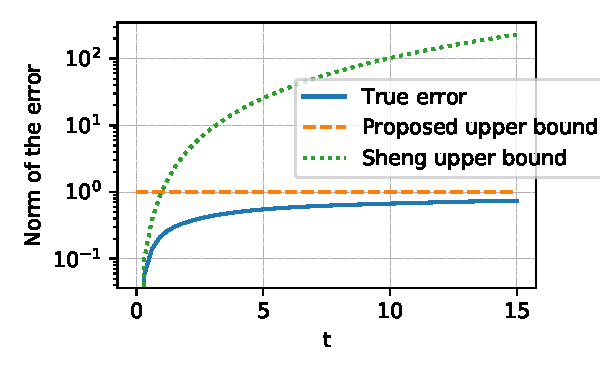
\includegraphics[width=\columnwidth]{upper_bound_2.pdf}}
\caption{Global error of the splitting scheme. Initial random full rank matrix $X \in \mathbb{R}^{100 \times 100}$ was splitted by rows. $X_1, X_2 \in \mathbb{R}^{50 \times 100}$. Target matrices were obtained the following way: $A_1 = -X_1^*X_1, A_2 = -X_2^*X_2, A = -X^*X$. So $A_1, A_2$ are negative and lacking full rank, while $A = A_1 + A_2$ has full rank.}
\label{strang:fig:upper_bound_2}
\end{center}
\vskip -0.2in
\end{figure}

% \begin{figure}[h!]
% 	\centering
% 	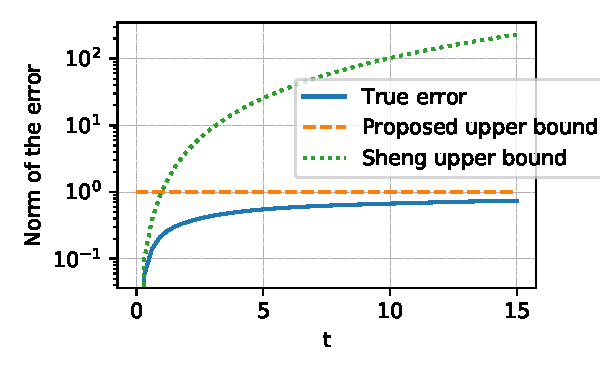
\includegraphics[width=0.6\textwidth]{upper_bound_2.pdf}
% 	\caption{Global error of the splitting scheme. Initial random full rank matrix $X \in \mathbb{R}^{100 \times 100}$ was splitted by rows. $X_1, X_2 \in \mathbb{R}^{50 \times 100}$. Target matrices were obtained the following way: $A_1 = -X_1^*X_1, A_2 = -X_2^*X_2, A = -X^*X$. So $A_1, A_2$ are negative and lacking full rank, while $A = A_1 + A_2$ has full rank.}
% 	\label{strang:fig:upper_bound_2}
% \end{figure}

The graph presented on the Figure \ref{strang:fig:upper_bound_2} describes . One can easily see significant difference between existing global upper bounds for that case \cite{sheng1994global} and derived upper bound.

\begin{theorem}\label{strang:theorem_uppbound}
	Let $A_1, A_2, \ldots, A_b \in \mathbb{S}^p_{+}$ be the square negative semidefinite matrices, that don't have full rank, i.e. $\operatorname{rank}{A_i} \leq p, \;\forall i = 1, \ldots, b$. While the sum of those matrices has full rank, i.e. $A = \sum\limits_{i=1}^b A_i, \operatorname{rank}{A} = p$. Then, the global upper bound error will be written as follows:

	\begin{equation}\label{strang:global_error_upper_bound}
		\lim_{t \to \infty}\| e^{A_bt} \cdot \ldots \cdot e^{A_1t} - e^{At}\| = \left\|\prod\limits_{i=1}^b \Pi_{b-i+1}\right\|,
	\end{equation}
	where $\Pi_i = I - Q_iQ_i^*$ and $A_i = Q_iB_iQ_i^*$ and $Q_i$ is a matrix with orthonormal columns. 
\end{theorem}

The graph on the Figure \ref{strang:fig:upper_bound_many} shows empirical validity of the presented upper bound.

\begin{figure}[ht]
\vskip 0.2in
\begin{center}
\centerline{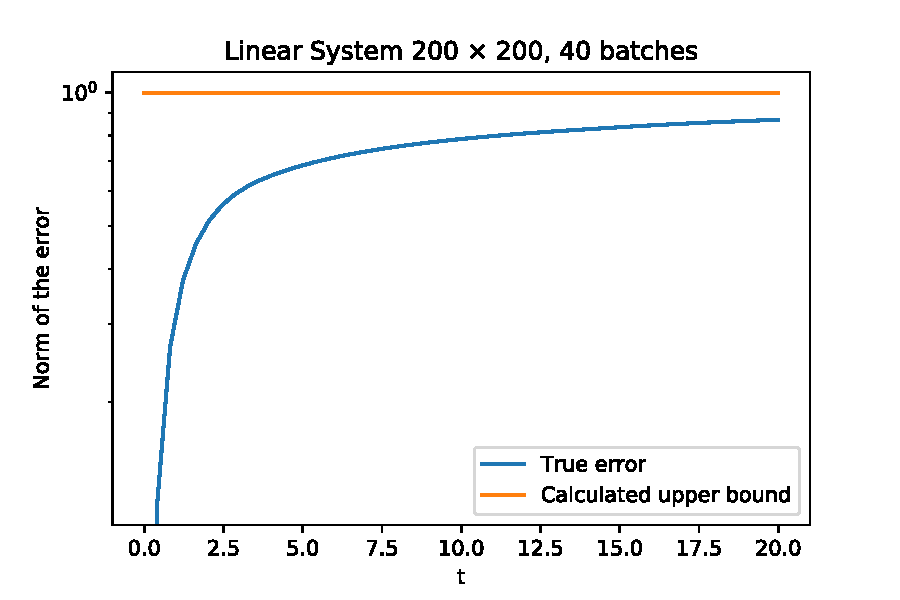
\includegraphics[width=\columnwidth]{upper_bound_many.pdf}}
\caption{Global upper bound on the splitting scheme in case of $40$ summands in the right-hand side.}
\label{strang:fig:upper_bound_many}
\end{center}
\vskip -0.2in
\end{figure}

\subsection{Binary logistic regression}
\subsubsection{Problem}
In this classification task then problem \eqref{strang:finitesum} takes the following form:
\begin{equation}\label{strang:LogReg}
-\frac{1}{n} \sum_{i=1}^n\left(y_i \ln \sigma(\vect{\theta}^\top\vect{x_i})  + (1-y_i) \ln (1-\sigma(\vect{\theta}^\top\vect{x_i}))\right) \to \min_{\vect{\theta} \in \mathbb{R}^p},
\end{equation}
where $\sigma(x) = \frac{1}{1 + e^{-x}}$ is the sigmoid function, while $ y_i \in \{0,1\}$ stands for the label of the object class.

\begin{equation}\label{strang:LogReg_grad}
\nabla_\theta f(\vect{\theta}) = \nabla f(\vect{\theta}) = \frac{1}{n}\sum\limits_{i=1}^n \vect{x_i}(\sigma(\vect{\theta}^\top\vect{x_i}) - y_i)
\end{equation}

The gradient flow equation will be written as follows:
\begin{equation}\label{strang:LogReg_GF}
\frac{d \vect{\theta}}{d t} = - \frac{1}{n}\sum\limits_{i=1}^n \vect{x_i}(\sigma(\vect{\theta}^\top\vect{x_i}) - y_i)
\end{equation}

Our particular interest lies in mini-batch reformulation of the given problem. We consider $s$ mini-batches with size $b$ regrouping ($b \cdot s = n$): $X_i \in \mathbb{R}^{b \times p}, \vect{y_i} \in \mathbb{R}^{b}$ and  $\sigma(\vect{x})$ stands for the element-wise sigmoid function.

\begin{equation}\label{strang:LogReg_GF_batch}
\frac{d \vect{\theta}}{d t} = - \frac{1}{n}\sum\limits_{i=1}^s X_i^\top\left(\sigma\left(X_i\vect{\theta}\right) - \vect{y_i}\right)
\end{equation}

\subsubsection{Splitting scheme and local problem}

Since we are applying splitting scheme to find the approximate solution of the \eqref{strang:LogReg_GF_batch}, each local problem should be written as follows:

\begin{equation}\label{strang:LogReg_GF_local}
\frac{d \vect{\theta}}{d t} =  - \frac{1}{n} X_i^\top\left(\sigma\left(X_i\vect{\theta}\right) - \vect{y_i}\right)
\end{equation}

Note, that this is not linear equation and cannot be solved as easy as in Theorem \ref{strang:LLS_local_solution}. However, we can apply the same technique to reduce the dimension of ODE, which is needed to be solved numerically. 

Suppose, we have $QR$ decomposition of each batch data matrix $X_i^\top = Q_i R_i$, then we can multiply both sides of \eqref{strang:LogReg_GF_local} on the $(I - Q_iQ_i^\top)$ on the left. 

\begin{align}
\nonumber (I - Q_iQ_i^\top)\frac{d \vect{\theta}}{d t} &= (I - Q_iQ_i^\top) \frac{1}{n} X_i^\top(\vect{y_i} -\sigma\left(X_i\vect{\theta}\right)) \\
\nonumber \frac{d \vect{\theta}}{d t} &= Q_i\frac{d (Q_i^\top\vect{\theta})}{d t} \quad Q_i^\top \vect{\theta} = \vect{\eta_i}\\ 
\nonumber \frac{d \vect{\theta}}{d t} &= Q_i\frac{d \vect{\eta_i}}{d t} \quad \text{integrate from $0$ to $h$}\\ 
\label{strang:logreg_theta_from_eta}\vect{\theta}(h) &= Q_i \left(\vect{\eta_i}(h) - \vect{\eta_i}(0) \right) + \vect{\theta}_0
\end{align}

On the other hand:
\begin{align}\nonumber
\frac{d \vect{\eta_i}}{d t} &= Q_i^\top\frac{d \vect{\theta}}{d t} =  - \frac{1}{n} Q_i^\top  X_i^\top(\sigma\left(X_i\vect{\theta}\right) - \vect{y_i}) = \\ 
\nonumber&= - \frac{1}{n} Q_i^\top  Q_i R_i(\sigma\left(X_i\vect{\theta}\right) - \vect{y_i}) =\\
\nonumber&= - \frac{1}{n} R_i(\sigma\left(X_i\vect{\theta}\right) - \vect{y_i})
\end{align}

Recall, that each hypothesis function depends on linear function $\vect{x_i}^\top \vect{\theta}$, which means, that in batch reformulation it is just entries of the vector $X_i \vect{\theta}$. Since we have $QR$ decomposition of $X_i^\top$, we can write: $X_i \vect{\theta} = R_i^\top Q_i^\top \vect{\theta} = R_i^\top \vect{\eta_i}$. In other words:

\begin{equation}
\label{strang:logreg_eta_ode}
\frac{d \vect{\eta_i}}{d t} = - \frac{1}{n} R_i\left(\sigma\left(R_i \vect{\eta_i}\right) - \vect{y_i}\right),
\end{equation}

To sum it up, we need to solve \eqref{strang:logreg_eta_ode} (which is much simpler, than original differential equation \eqref{strang:LogReg_GF_local}), than substitute it to the
\eqref{strang:logreg_theta_from_eta} with $\vect{\eta_i}(0) = Q_i^\top \vect{\theta}_0$. Note, that matrices $Q_i$ and $R_i$ can be computed only once before the training.
\subsection{Softmax regression}
\begin{equation*}
\end{equation*}
\subsection{Problem}

%================================================
% Results
%============================={}===================

\section{Results}
\subsection{Iteration comparison}
\subsection{Time comparison}
\subsection{Robustness to stepsize choosing}

\subsubsection{Linear Least Squares}

\begin{figure}[ht]
\vskip 0.2in
\begin{center}
\centerline{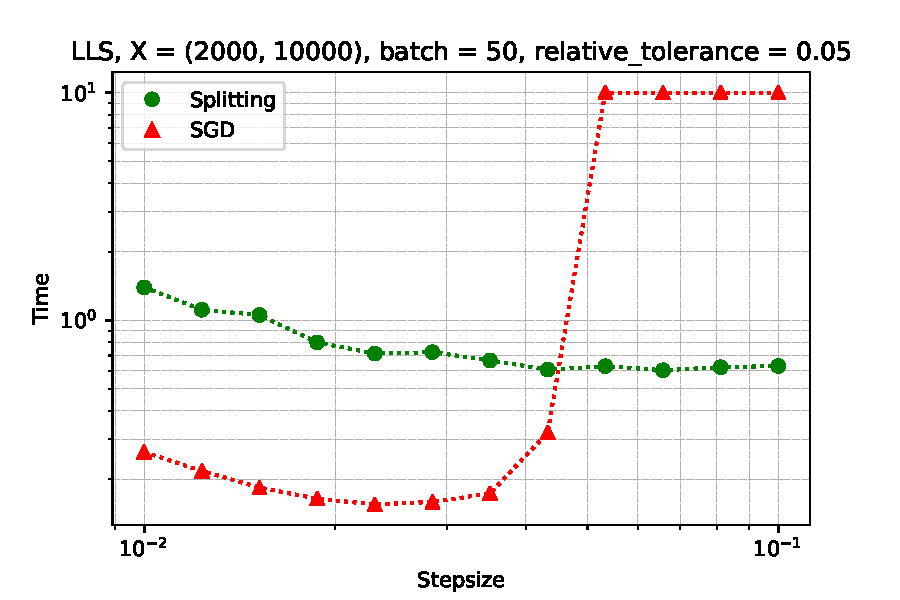
\includegraphics[width=\columnwidth]{sgd_split_iterations_lls.pdf}}
\caption{Random linear system. Averaging on 30 runs.}
\label{strang:fig:lls_step_iter}
\end{center}
\vskip -0.2in
\end{figure}

\begin{figure}[ht]
\vskip 0.2in
\begin{center}
\centerline{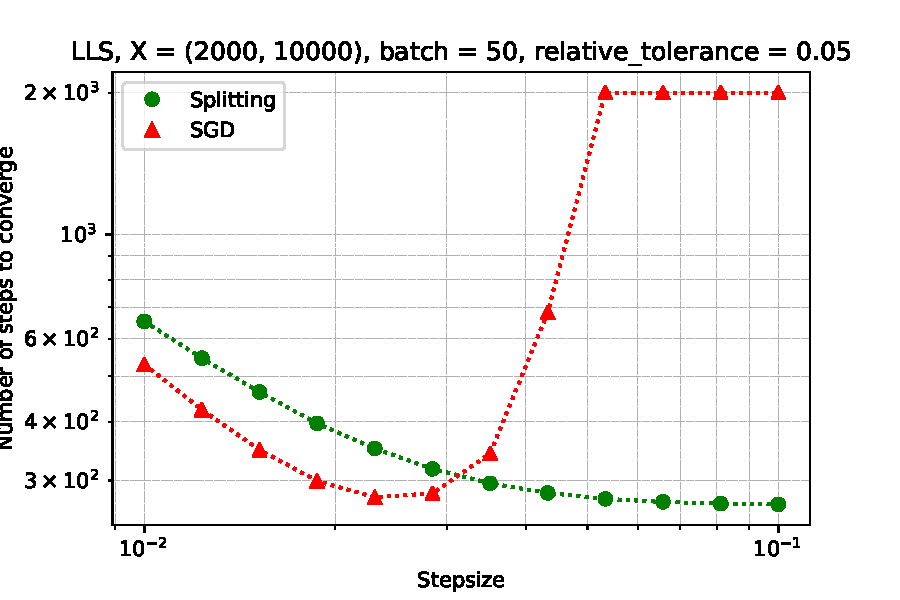
\includegraphics[width=\columnwidth]{sgd_split_time_lls.pdf}}
\caption{Random linear system. Averaging on 30 runs.}
\label{strang:fig:lls_step_time}
\end{center}
\vskip -0.2in
\end{figure}

\subsubsection{Binary Logistic Regression}

\begin{figure}[ht]
\vskip 0.2in
\begin{center}
\centerline{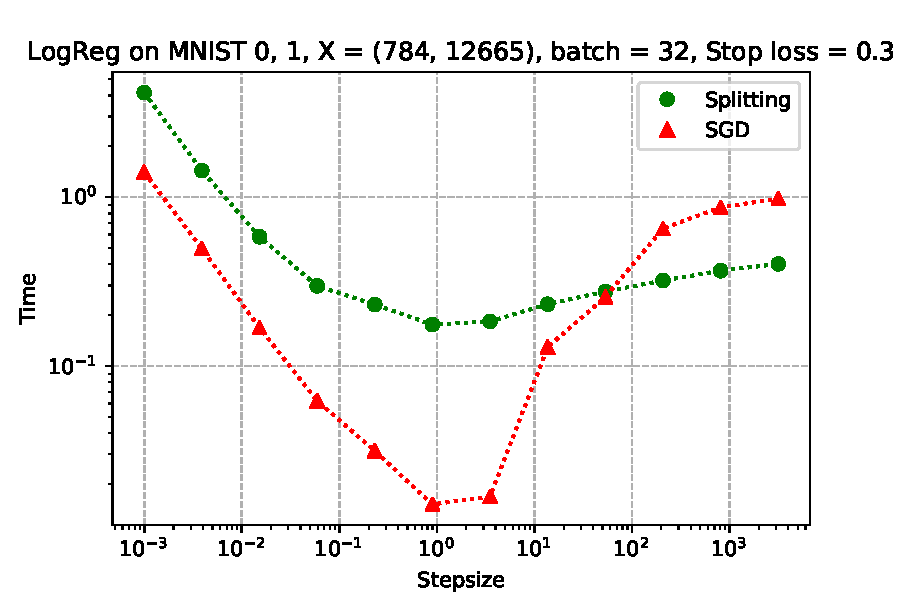
\includegraphics[width=\columnwidth]{sgd_split_iterations_logreg.pdf}}
\caption{MNIST 0,1. Binary logistic regression. Averaging on 30 runs}
\label{strang:fig:logreg_step_iter}
\end{center}
\vskip -0.2in
\end{figure}

\begin{figure}[ht]
\vskip 0.2in
\begin{center}
\centerline{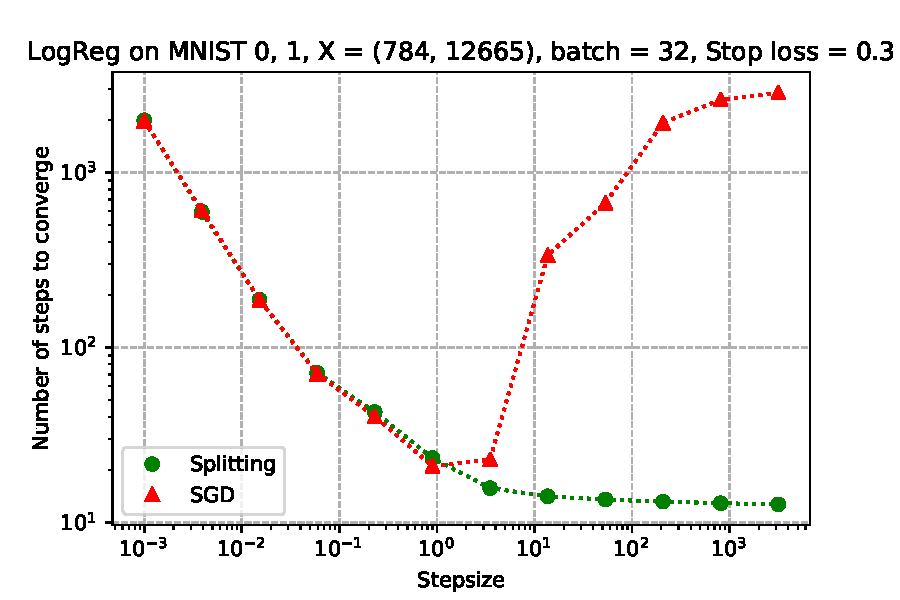
\includegraphics[width=\columnwidth]{sgd_split_time_logreg.pdf}}
\caption{MNIST 0,1. Binary logistic regression. Averaging on 30 runs}
\label{strang:fig:logreg_step_time}
\end{center}
\vskip -0.2in
\end{figure}

%================================================
% Related work
%================================================

\section{Related work}

In \cite{su2014differential} authors introduced second order ODE, which is equivalent (in the limit sense) to the gradient descent with Nesterov momentum \cite{nesterov1983method}. The paper contains both formal and intuitive derivation of the proposed ODE from the iterative method itself with analogous upper bounds for general convex optimization setting and closed form solution for quadratic function. Strongly convex and composite optimizations are also covered. Theoretical conclusions are supported by strong empirical results on the variety of test functions.

Generalization of these ideas were presented in \cite{wibisono2016variational} with an arbitrary polynomial acceleration using the same parameter in ODE.

Solution dynamics of the linear least squares problem was also studied in \cite{osher2016sparse} based on the linearized Bregman iteration.

General overview of interplay between continuous-time and discrete-time point of views on dynamical systems and iterative optimization methods is covered in \cite{helmke2012optimization}, \cite{evtushenko1994stable}

\newpage
\bibliography{biblio}
\bibliographystyle{icml2020}


%%%%%%%%%%%%%%%%%%%%%%%%%%%%%%%%%%%%%%%%%%%%%%%%%%%%%%%%%%%%%%%%%%%%%%%%%%%%%%%
%%%%%%%%%%%%%%%%%%%%%%%%%%%%%%%%%%%%%%%%%%%%%%%%%%%%%%%%%%%%%%%%%%%%%%%%%%%%%%%
% DELETE THIS PART. DO NOT PLACE CONTENT AFTER THE REFERENCES!
%%%%%%%%%%%%%%%%%%%%%%%%%%%%%%%%%%%%%%%%%%%%%%%%%%%%%%%%%%%%%%%%%%%%%%%%%%%%%%%
%%%%%%%%%%%%%%%%%%%%%%%%%%%%%%%%%%%%%%%%%%%%%%%%%%%%%%%%%%%%%%%%%%%%%%%%%%%%%%%

%================================================
% Appendix
%================================================

\appendix
\section{Proofs}
\section{Additional graphs}


\begin{figure}
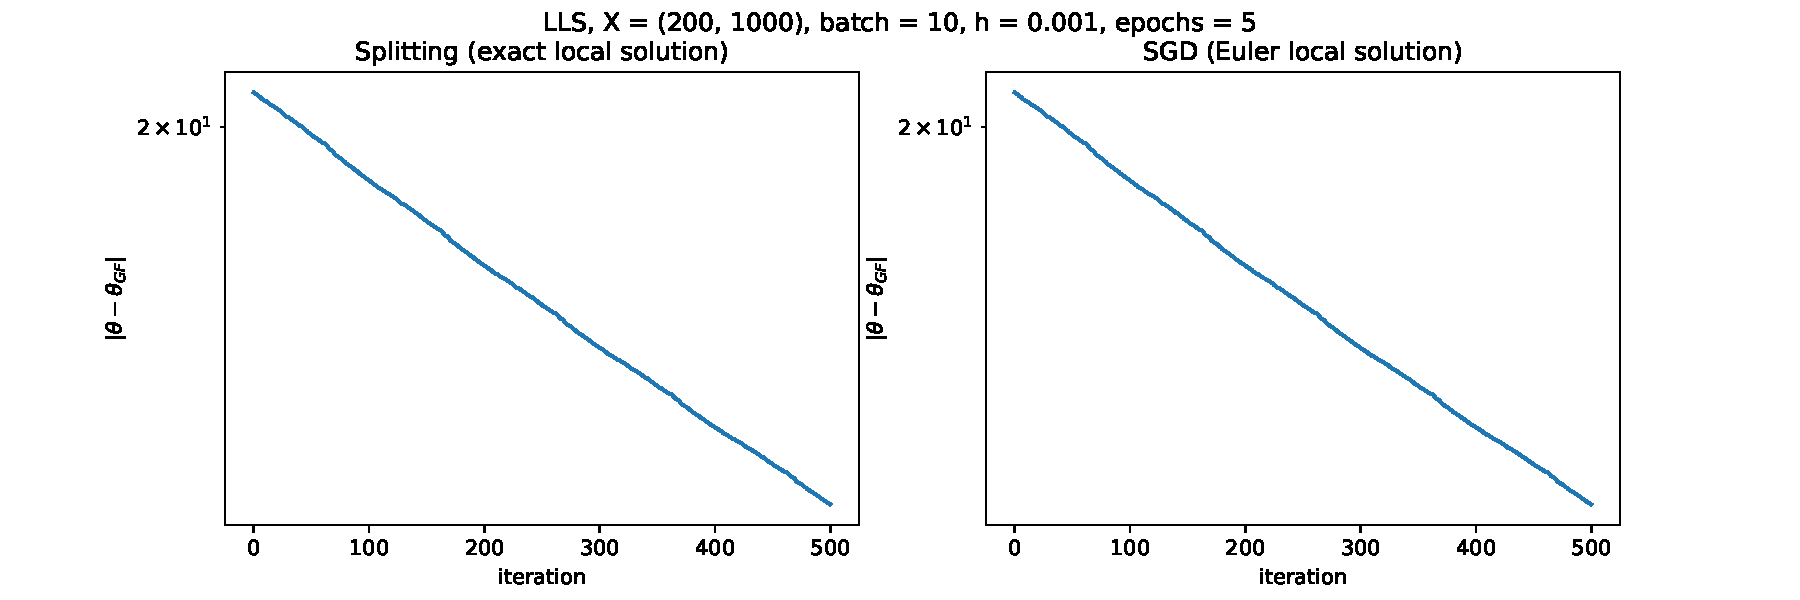
\includegraphics[width=0.85\textwidth]{{robustness_to_stepsize/sgd_split0.001}.pdf} \\
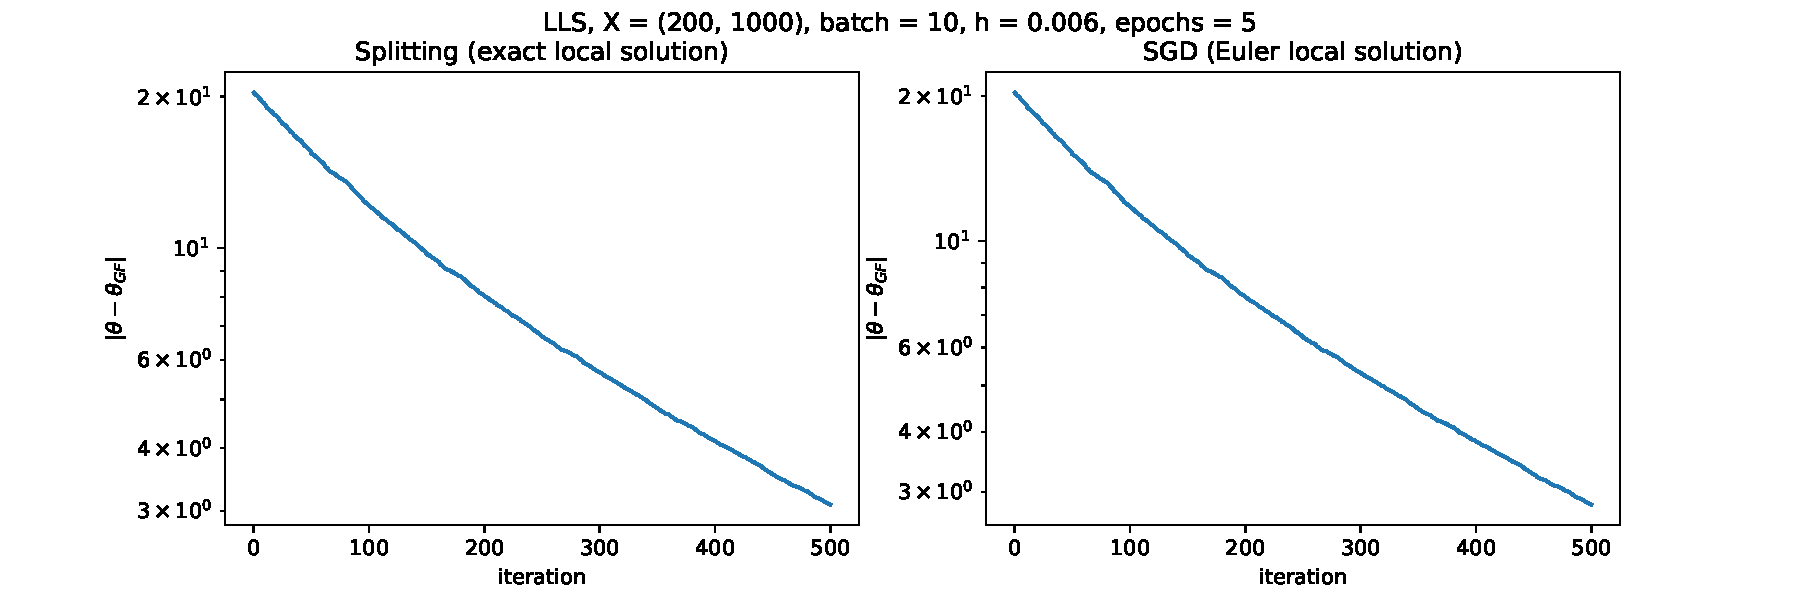
\includegraphics[width=0.85\textwidth]{{robustness_to_stepsize/sgd_split0.006}.pdf} \\
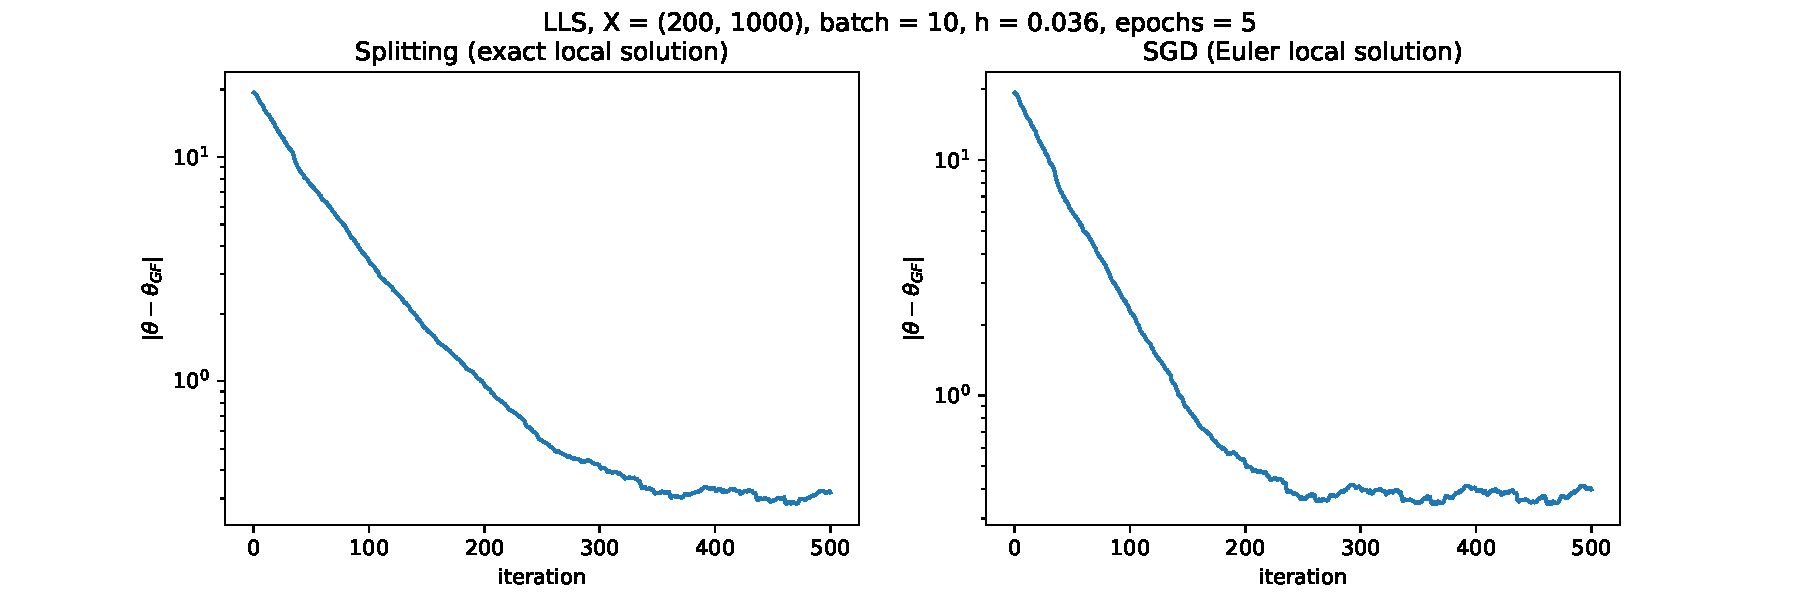
\includegraphics[width=0.85\textwidth]{{robustness_to_stepsize/sgd_split0.036}.pdf} \\
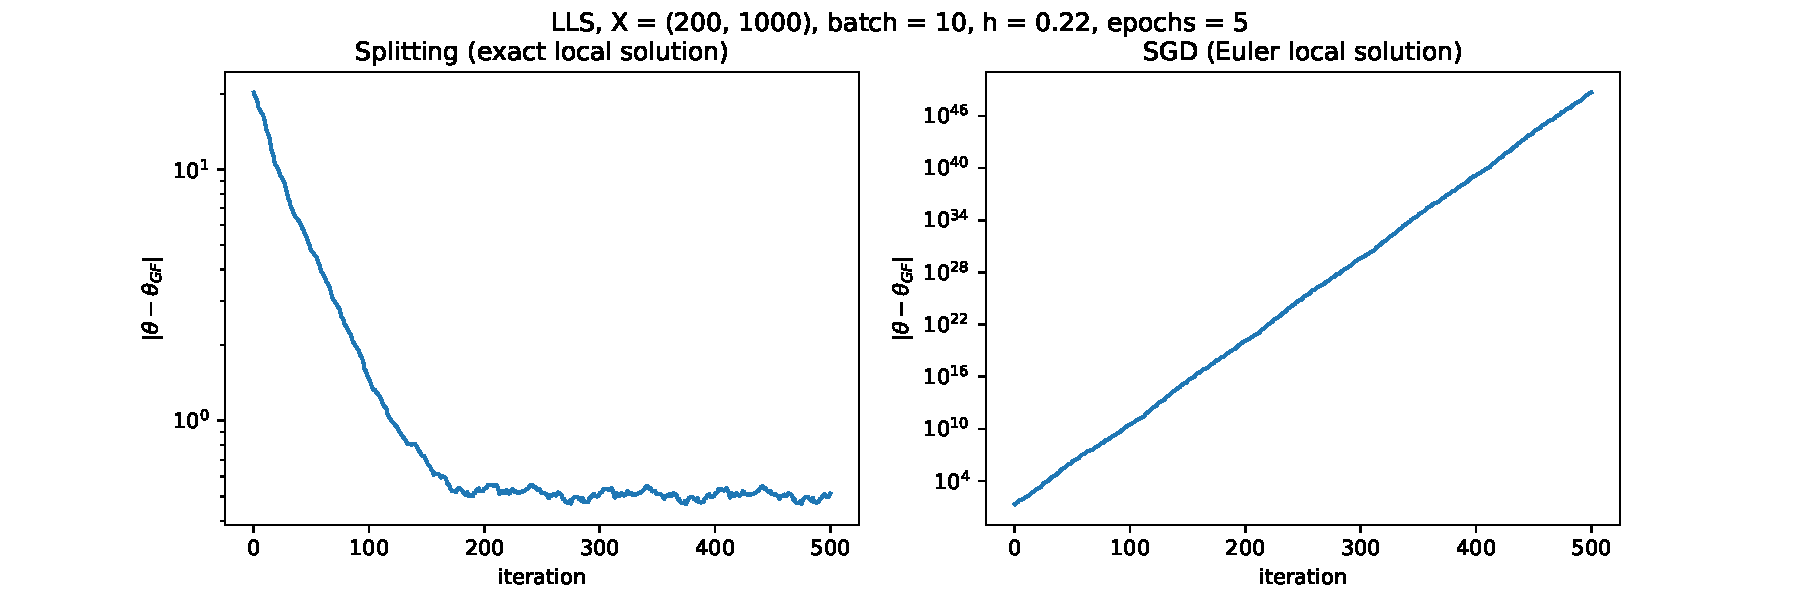
\includegraphics[width=0.85\textwidth]{{robustness_to_stepsize/sgd_split0.22}.pdf} \\
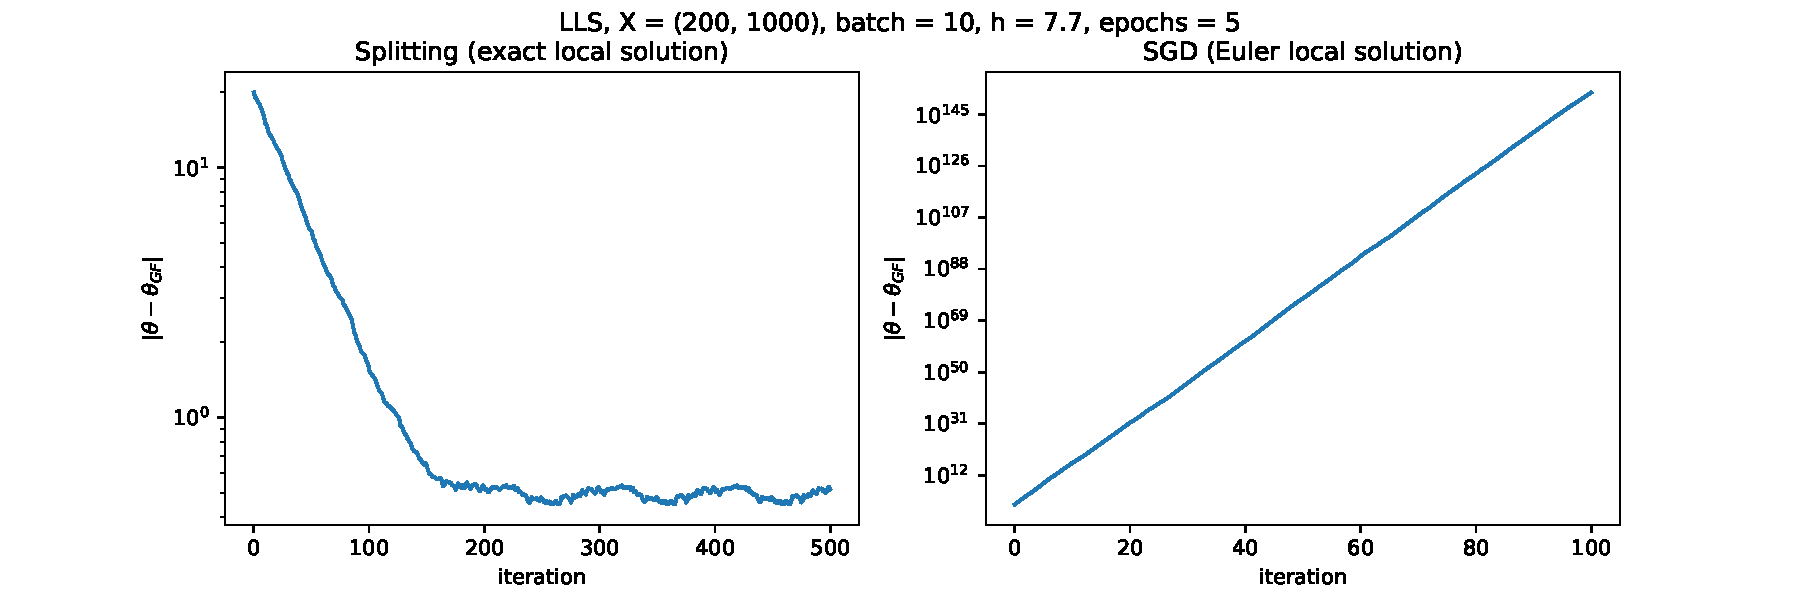
\includegraphics[width=0.85\textwidth]{{robustness_to_stepsize/sgd_split7.7}.pdf} \\
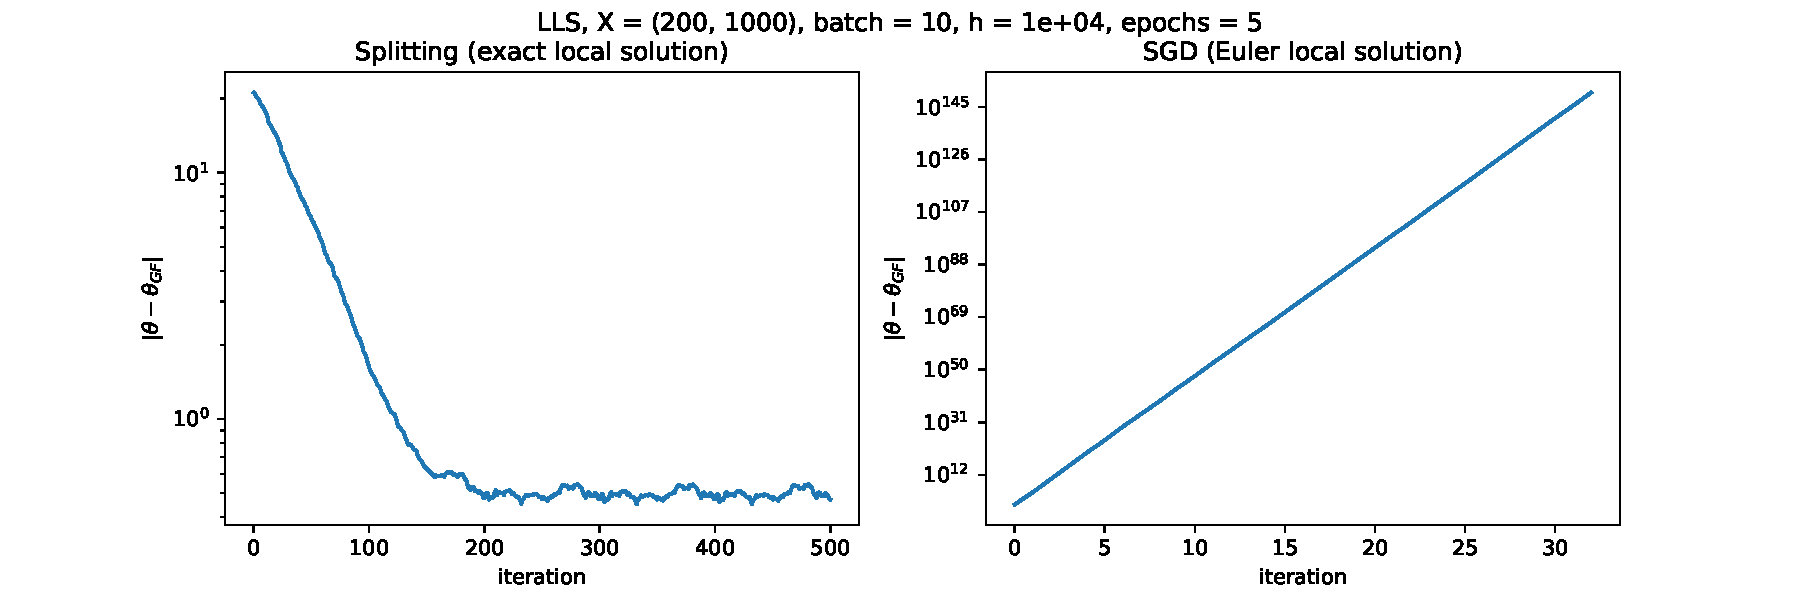
\includegraphics[width=0.85\textwidth]{{robustness_to_stepsize/sgd_split1e+04}.pdf}
\caption{Linear Least Squares, $X \in \mathbb{R}^{200 \times 1000}, b = 10$}
\end{figure}


\begin{figure}
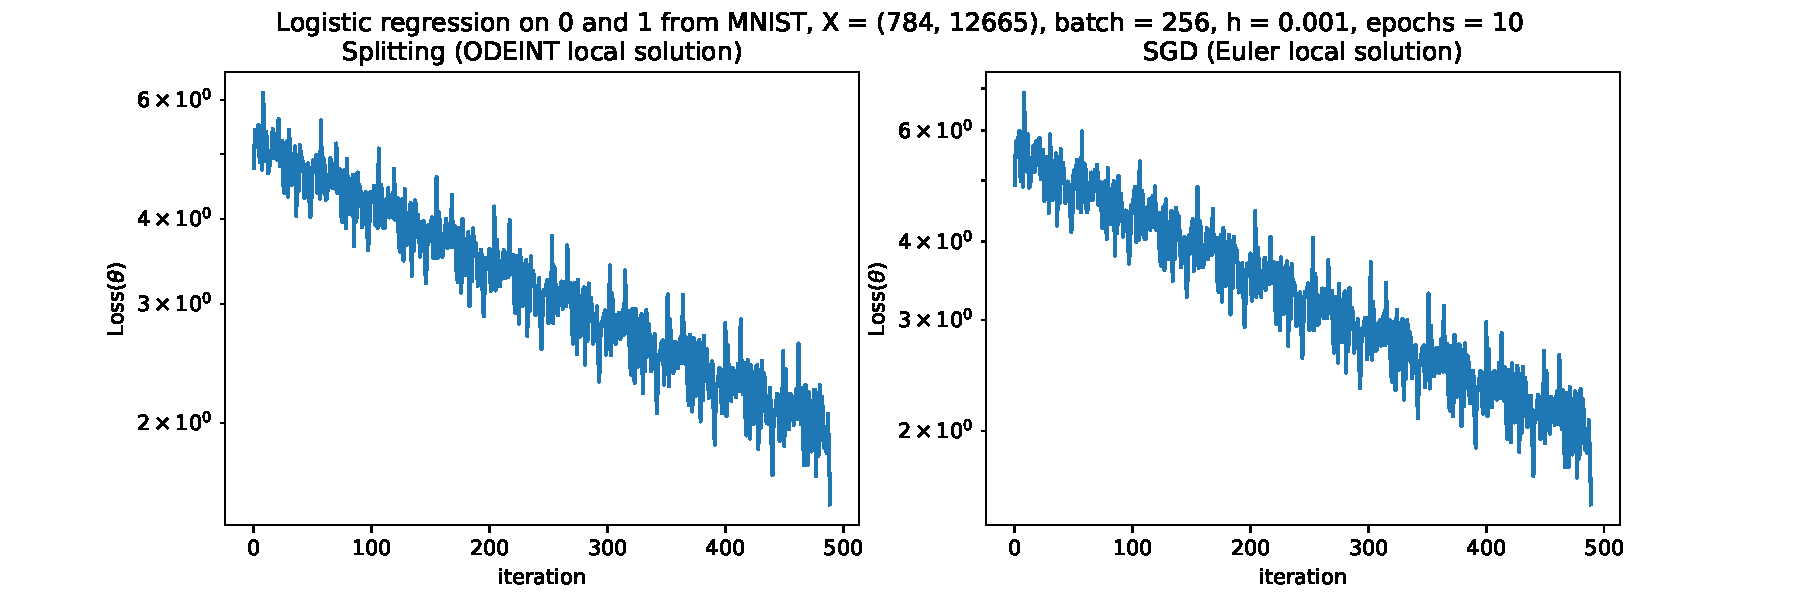
\includegraphics[width=0.85\textwidth]{{robustness_to_stepsize/sgd_split_logreg0.001}.pdf} \\
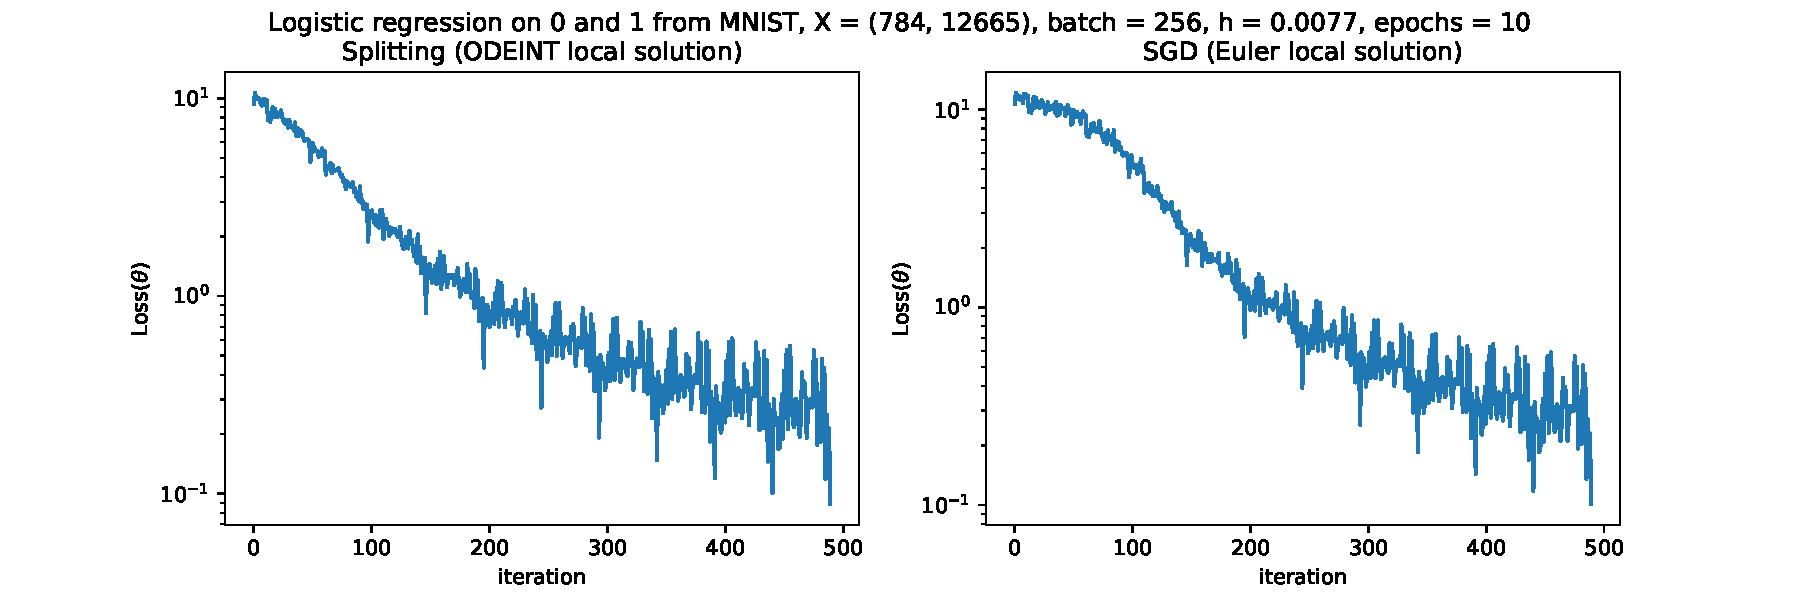
\includegraphics[width=0.85\textwidth]{{robustness_to_stepsize/sgd_split_logreg0.0077}.pdf} \\
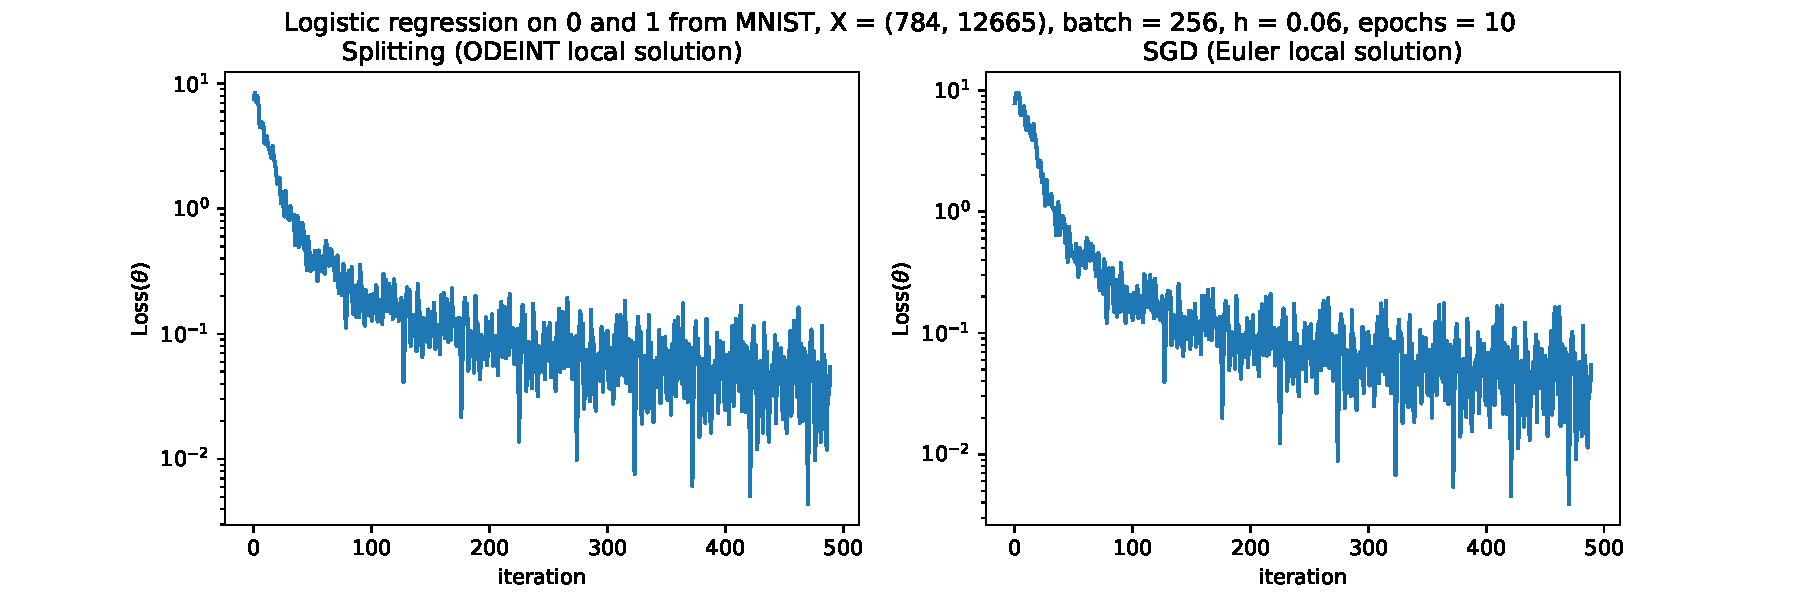
\includegraphics[width=0.85\textwidth]{{robustness_to_stepsize/sgd_split_logreg0.06}.pdf} \\
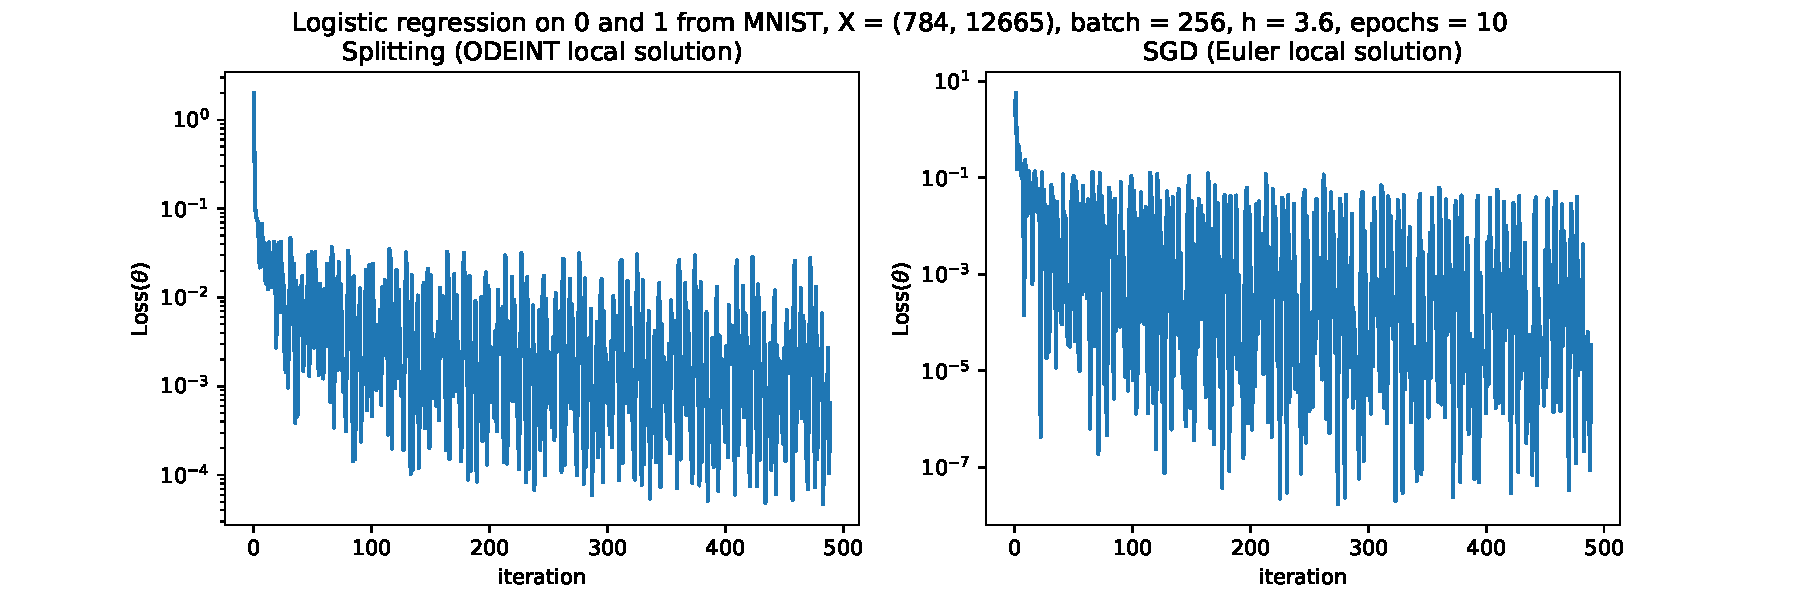
\includegraphics[width=0.85\textwidth]{{robustness_to_stepsize/sgd_split_logreg3.6}.pdf} \\
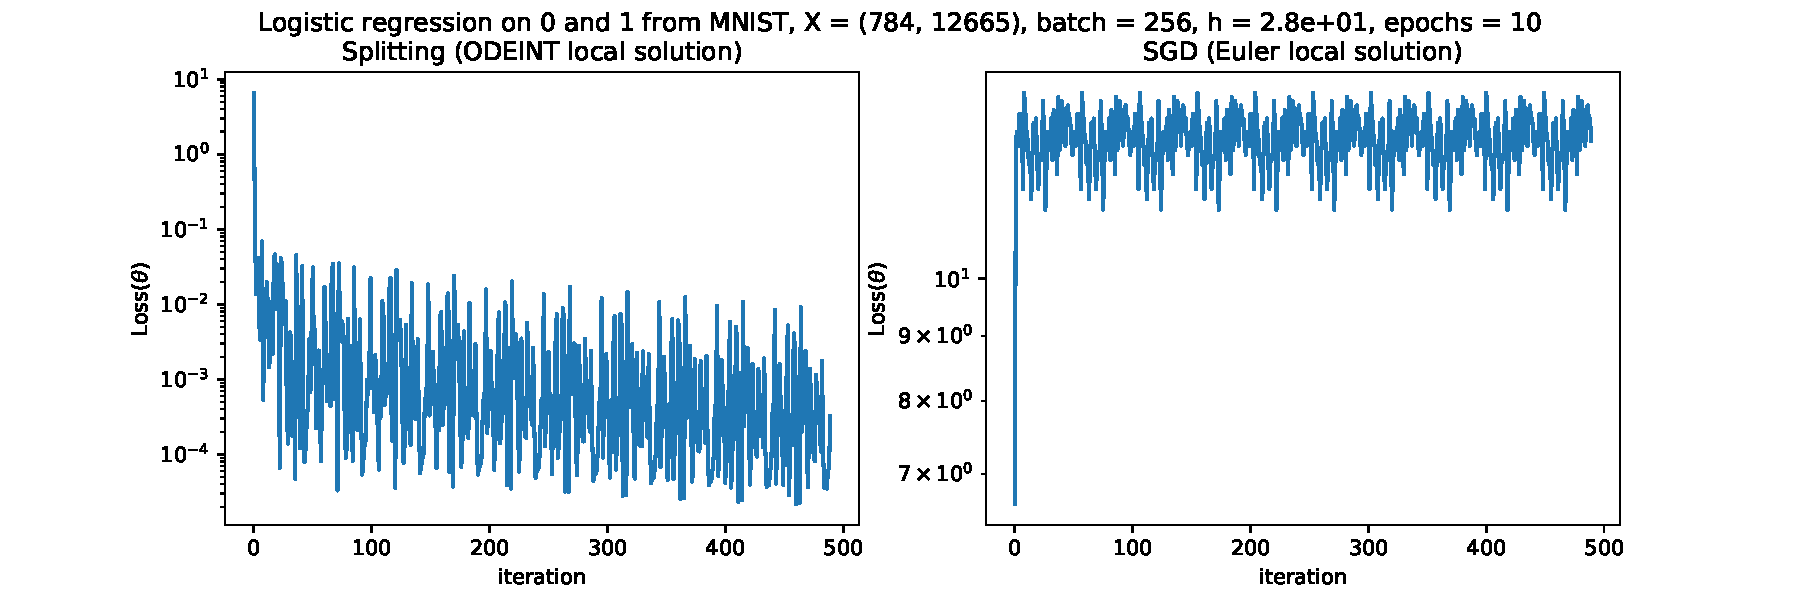
\includegraphics[width=0.85\textwidth]{{robustness_to_stepsize/sgd_split_logreg2.8e+01}.pdf} \\
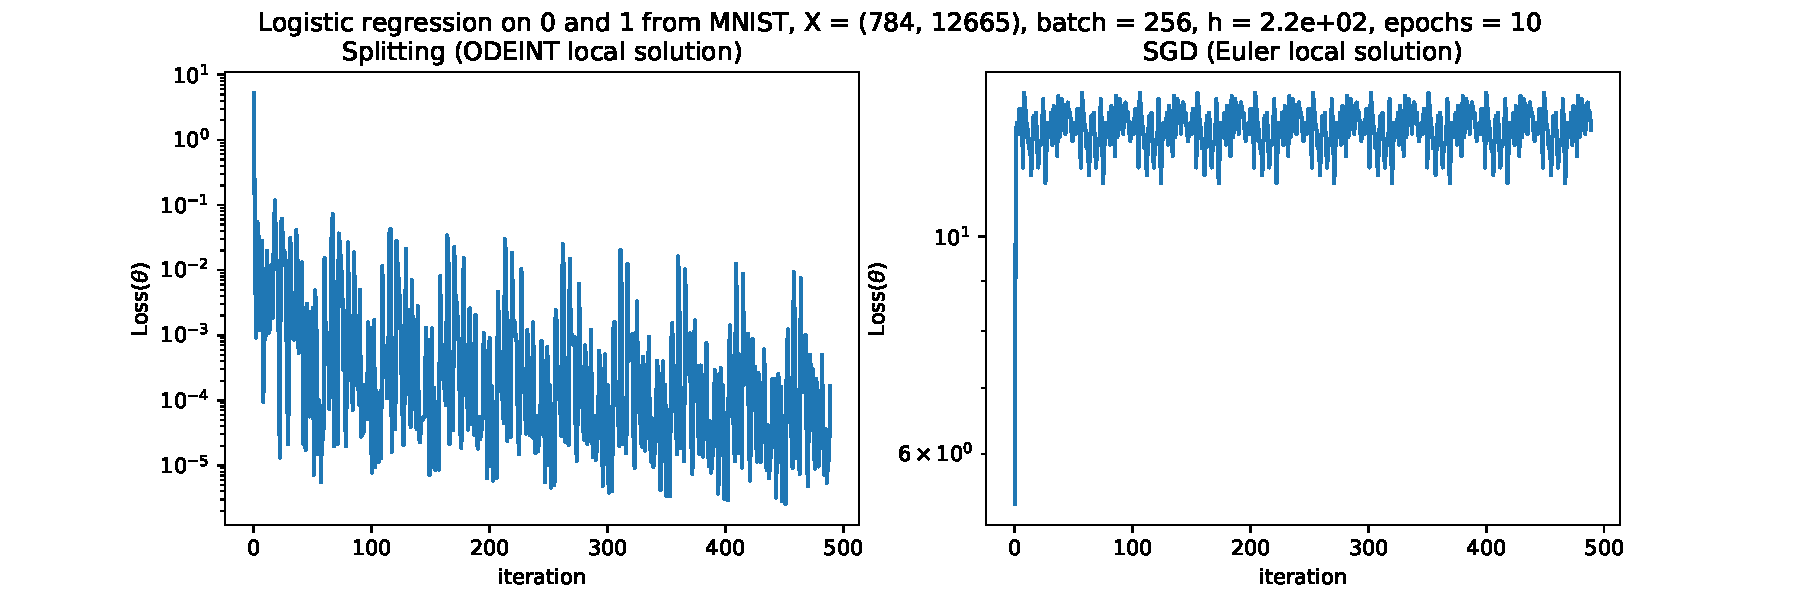
\includegraphics[width=0.85\textwidth]{{robustness_to_stepsize/sgd_split_logreg2.2e+02}.pdf}
\caption{Binary logistic regression on 0 and 1 from MNIST dataset}
\end{figure}

\end{document}